\chapter{对象与类}\label{chap:class}

本章将会讨论“对象”和“类”的思想在高中理科中的应用。

我们知道等式的一个基本原则: \textbf{等号两边的内容必须相等}。这句话不仅表明两边
的数值相等,还指出两边的东西应该是\emph{同类的}——三个苹果不能等于三棵树。在高中
理科的学习中,这种“同类”的思想经常出现。

\section{量纲分析}

\subsection{单位、单位的运算}

在物理必修一第四章第4节,我们学习了国际单位制(SI)\index{国际单位制}。SI的七个
基本单位如表~\ref{tbl:si_units}~所示。

\begin{table}[ht]
    \centering
    \caption{SI的基本单位}\label{tbl:si_units}\index{国际单位制!基本单位}
    \begin{tabular}{cccc}
        \toprule
        物理量 & 物理量符号 & 单位 & 单位符号 \\
        \midrule
        长度 & $l$ & 米 & \unit{m} \\
        质量 & $m$ & 千克 & \unit{kg} \\
        时间 & $t$ & 秒 & \unit{s} \\
        电流 & $I$ & 安培 & \unit{A} \\
        热力学温度 & $T$ & 开尔文 & \unit{K} \\
        物质的量 & $n$ & 摩尔 & \unit{mol} \\
        发光强度 & $I$ & 坎德拉 & \unit{cd} \\
        \bottomrule
    \end{tabular}
\end{table}

这七个物理量的现代定义都是基于某个已知的常量。比如,秒的定义用到了铯-133原子跃迁
所释放辐射的周期;而米的则用到了光速和秒。

一些物理概念是没有单位的,比如物体的个数、用弧度表示的角等。

物理量的运算同时伴随的单位的运算。人们常说,你不能把苹果和橙子相加(You 
can't add apples and oranges),指的是\textbf{单位不同的物理量不能直接相加}。也
就是说,只有相同单位的物理量可以相加。与加法不同的是,乘法并不要求物理量的单位相
同:
\begin{gather*}
    \qty{2}{\meter} \times \qty{3}{\meter} = \qty{6}{\meter^2},\\
    \qty{4}{\meter} \times \qty{2}{\second} = \qty{8}{\meter\cdot\second},\\
    \frac{\qty{4}{\coulomb}}{\qty{2}{\mole}} = \qty{2}{\coulomb\per\mole}.\\
\end{gather*}

在基本和导出单位名称之前加上词头,可表达该单位的倍数和分数,一般都是$10$的整数幂。
比如,词头kilo(千,前缀k)表示$10^3$;nano(纳,前缀n)则表示$10^{-9}$。这样一
来,\unit{\kilo\mol}表示~\qty{e3}{\mol};\unit{\nano\A}则表示~\qty{e-9}{\A}。

在形式上,一个带单位的物理量一定程度上相当于“数值和单位的乘积”。比如:
\begin{gather*}
    \qty{2000}{s} = \qty{2e3}{s} = \qty{2}{\kilo\s},\\
    \qty{1800}{\km\cdot\s} = \qty{1.8}{\km\cdot\kilo\s} = \qty{1.8}
    {\mega\metre\cdot\s}
.\end{gather*} 

\subsection{导出单位}\index{国际单位制!导出单位}

SI的\textbf{导出单位}是基本单位在乘幂、乘积或相除后产生的单位。每一个导出单位都
与一个导出物理量相对应。

速度按照定义是长度与时间的比值,因此它的单位也是对应基本单位的商~\unit{\m\per\s};
力的单位牛顿\index{牛顿}的定义是“使1千克的\emph{质量}产生1米每二次方秒的\emph{加
速度}需要的力”,而质量和加速度在SI中对应的单位分别是~\unit{\kg}~和%
~\unit{\m\per\square\s},且根据$F=ma$,力是质量和加速度之积,所以力的单位牛顿就
为~\unit{\kg\m\per\square\s}。

\textbf{一致单位}\index{国际单位制!导出单位!一致单位}是指定义中系数均为1的导出单
位,也就是定义中不会出现像标准重力或是水的密度之类的常数。牛顿的定义中的系数都是%
1:“1千克”“1米每二次方秒”,不含其他数值,所以牛顿是一个一致单位。

一些导出单位也有自己的名称和符号,刚才提到的牛顿(\unit{\N})就是一个例子。此外
常见的导出单位还有焦耳(\unit{\J},\unit{\kg\square\m\per\square\s})、帕斯卡
(\unit{\Pa},\unit{\kg\per\m\per\square\s})、库仑(\unit{\C},\unit{\s\A})等。
\index{焦耳}\index{帕斯卡}\index{库仑}

\begin{rawexp}\label{exp:particle_density_unit}
    一个物理量表示的是某种粒子在单位体积的个数,它的SI单位是什么?
\end{rawexp}

\begin{rawsol}
    已知这种物理量(不妨记为$X$)的定义是
    \[
        X \coloneq \frac{\text{一些粒子的个数}}{\text{这些粒子占据了多少单位体积}}
    ,\]
    那么$X$应该是“个数/体积”,其单位为“个数”和“体积”单位的比,是~\unit{\m^{-3}}
    (由于“个数”没有SI单位)。
\end{rawsol}

\subsection{量纲}

我们知道,在物理学中,各种物理量有着不同的单位,这些单位之间却有一定的联系。通过合理地规定
一些基本单位(基本单位),可以将其他所有单位(导出单位)表示为这些基本单位的乘积,
从而统一各个物理量之间的关系。例如,在国际单位制中,功的单位是焦耳
(\si{\joule}),可以表示为“千克·平方米每平方秒”
(\si{\kilogram\meter\squared\per\second\squared})。

然而,仅仅用单位来表示物理量会带来一些问题:

\begin{enumerate}
    \item 在不同的单位制下,同一个物理量会有不同的表示方式,难以达到“统一各单位”
        的效果。例如,速度的单位在英里每小时(mph)和米每秒
        (\si{\meter\per\second})之间看似没有联系,但实际上都是速度的表示。尽管
        可以通过转换来统一基本单位,但这种方法既不直观,也不方便记忆,而且选择哪
        个单位作为统一标准也并不公平。
    
    \item 将现有单位拆分为基本单位的形式实际上没有意义。例如,功的单位不是“千克
        $\cdot$平方米每平方秒”,它只是恰好与“焦耳”相等而已。此外,这样做还会导致
        一些单位被拆分后相同但实际上不同的情况,如力矩的单位牛米
        (\si{\newton\meter})拆分后也是
        \si{\kilogram\meter\squared\per\second\squared},但显然它与功是完全不同
        的。
\end{enumerate}



因此,引入了量纲作为表达导出单位组成的专有方式,以解决上述问题。它表示物理量与基
本物理量(如长度、质量、时间、电流、温度、物质的量和光强度)的关系。量纲的表示通
常使用大写字母,例如:长度($\mathrm {L} $),质量($\mathrm {M} $),温度
($\Theta$),电流($\mathrm {I} $),时间($\mathrm{T}$),物质的量($\mathrm 
{N} $),发光强度($\mathrm {J} $)。这些基本量纲可以组合形成复合量纲。

一个物理量$X$的量纲用$\dim X$表示。\index{$\dim X$}

和单位不同的是,一个物理量的量纲是唯一的。比如,速度的单位可能有“米每秒”“英里每
分钟”或“光年每年”,但是速度的量纲只有$\mathrm{LT^{-1}}$这一个。

SI中的一致单位\index{一致单位}的导出表达和量纲在形式上应该是相似的,因为两者都没
有额外的常数干扰。

\subsection{量纲分析}

\begin{rawthm}
    在物理公式中,等号左右应该在谈论同一个物理量。因此,等号左右的量纲是相等的。
\end{rawthm}

这个定理可以帮助我们推导新物理量的单位(SI导出单位形式)、判断公式的正确性以及推
导新的公式,让我们逐个举例看看。

\subsubsection{推导物理量单位}

下面的推导过程得出了电压这一物理量的量纲:
\begin{align*}
    U &= \frac{P}{I} = \frac{W\cdot t}{I} = \frac{Fxt}{I},\\
    \dim U &= \dim \left( \frac{Fxt}{I} \right) \\
                      &= \frac{\dim (Fxt)}{\dim I} \\
                      &= \mathrm{L^2MT^{-3}I^{-1}}
.\end{align*} 

所以相应地,伏特这一单位与~\unit{\square\m\kg\per\cubic\s\per\A}~是一致的。

\subsubsection{验证公式正确性}

我们学过电流的微观表达式$I=nvqS$,其中$S$表示导体的横截面积,$n$表示在导体中的载
流子密度(单位体积内载流子个数),$v$表示导体中载流子垂直于横截面的速度大小,$q$
表示导体中每个载流子的电荷量。这个公式是否正确?我们可以试试量纲分析。

也许你发现了,$n$就相当于例~\ref{exp:particle_density_unit}~中提及的物理量,它的
单位应是~\unit{\per\cubic\meter},量纲则是$\mathrm{L^{-3}}$。此外,$S$的量纲是
$\mathrm{L^2}$;$v$的是$\mathrm{LT^{-1}}$;$q$的是$\mathrm{TI}$。

将它们相乘我们得到了
\[
    \dim (vnqS) = \mathrm{LT^{-1}\cdot L^{-3}\cdot TI\cdot L^2 = I }
.\] 

物理量乘积$vnqS$的量纲是$\mathrm{I}$,恰好是电流,可见这个公式是正确的。

\subsubsection{推导新公式}

我们在推导单摆的周期公式时,可以先猜测其周期$T$与摆长$l$、摆重$m$和重力加速度$g$
有关,于是我们假设
\[
    T = \lambda m^{x}l^{y}g^{z}   
.\]
其中$\lambda $是一个比例常数。

左右同时取量纲,我们得到
\[
    \mathrm{T} = \mathrm{M}^{x}\mathrm{L}^{y}\left( \mathrm{LT}^{-2} \right)^{z} 
.\] 

根据左右量纲相等,得到
\[
    \begin{cases}
        0=y+z,\\
        0=x,\\
        -2z=1.
    \end{cases}
\] 
解得$x=0,y=\frac{1}{2},z=-\frac{1}{2}$,所以有
\[
    T = \lambda \sqrt{\frac{l}{g}} 
.\] 
只需进行实验测出$\lambda$即可。

\subsubsection{例题与练习}

学会了量纲分析的思想,在面对一些以往看似复杂的“求表达式”的题目时往往可以更加方便。

\begin{rawexp}\label{exp:current_expl}
    一根横截面积为$S$的均匀长直橡胶棒上均匀带有负电荷,每米橡胶棒所带电荷量为$q$,
    当此棒沿轴线方向做速度为$v$的匀速直线运动时,由于棒的运动而形成的等效电流大
    小为\choiceblank。

    \begin{tasks}(4)
        \task $vq$
        \task $\frac{q}{v}$
        \task $qvS$
        \task $\frac{qv}{S}$
    \end{tasks}
\end{rawexp}

\begin{rawsol}
    选A。我们先分析题目中几个物理量的物理意义,以此得出其量纲。

    \begin{table}[H]
        \centering
        \begin{tabular}{cccc}
            \toprule
            物理量 & 物理意义 & 国际单位 & 量纲 \\
            \midrule
            $S$ & 棒的横截面积 & \unit{\square\metre} & $\mathrm{L^2}$ \\
            $q$ & 每米橡胶棒所带电荷量 & \unit{\coulomb\per\metre} & 
            $\mathrm{ITL^{-1}}$ \\
            $v$ & 棒的宏观速度 & \unit{\meter\per\second} & $\mathrm{LT^{-1}}$ 
            \\
            \bottomrule
        \end{tabular}
    \end{table}
    
    接下来,我们有两种方法:逐个代入,检查每个选项的量纲;或类似单摆周期的例子,
    列方程组求解各物理量的次数。我们用第一种方法。

    题目要求的结果的量纲为$\mathrm{I}$。 A选项的量纲是$\mathrm{LT\cdot%
    IT^{-1}L^{-1} = I}$,满足题意。类似地,B选项的量纲是$\mathrm{IT^2L^{-2}}$;C
    选项的量纲是$\mathrm{IL^2}$;D选项的量纲是$\mathrm{IL^{-2}}$,均不符合题意。
    故选A。
\end{rawsol}

可以看出,在熟练掌握之后,用这种量纲分析的思想确实可以轻松解决部分题目。用此方法
的关键在于正确判断题目中物理量的物理意义及其量纲(或单位)。例题~\ref{exp:current_expl}~中
的$q$并非传统意义上的“电荷量”,而是“单位长度(每米)所带的电荷量”。所以,其单位
也应为~\unit{\coulomb\per\m}~而非~\unit{\C}。


\begin{exercises}
\item 辐射的危害程度常用“当量剂量”这一物理量衡量,其国际单位是希沃特(西弗),记作
    ~\unit{Sv}。每千克人体组织吸收1焦耳为1希沃特。下列选项中用国际单位制的基本单
    位表达希沃特,正确的是\choiceblank。
    \begin{tasks}(4)
        \task \unit{\square\m\per\square\s}
        \task \unit{\W\per\kg}
        \task \unit{\J\per\kg}
        \task \unit{\square\m\per\s}
    \end{tasks}

\item 2018年,国际基本单位之一“千克”被重新定义为:一千克等于普朗克常量$h$除以
    \qty{6.62607015e-34}{\square\m\per\s},则普朗克常量$h$的单位是\choiceblank。
    \begin{tasks}(2)
        \task \unit{\kg\s\per\square\m}
        \task \unit{\kg\square\m\per\s}
        \task \unit{\square\m\per\kg\per\s}
        \task \unit{\square\m\s\per\kg}
    \end{tasks}

\item 匀强电场中有一与电场垂直的平面,面积为$S$,该电场的电场强度随时间的变化率
    为$\frac{\Delta E}{\Delta t}$,静电力常量为$k$,则$\frac{1}{4 \pi k}
    \cdot\frac{\Delta E}{\Delta t}S$对应物理量的单位是\choiceblank。
    \begin{tasks}(4)
        \task 欧姆
        \task 伏特
        \task 瓦特
        \task 安培
    \end{tasks}

\item 声音在空气中的传播速度$v$与空气的密度$\rho $、压强$p$有关,下列速度表达式中
    $K$为比例系数,无单位,则这四个表达式中可能正确的是\choiceblank。
    \begin{tasks}(2)
        \task $v=\frac{Kp}{\rho }$
        \task $v=\sqrt{\frac{Kp}{\rho }} $
        \task $v=\sqrt{\frac{K \rho }{p}} $
        \task $v=\sqrt{K \rho p} $
    \end{tasks}

\item 由相关电磁学知识可以知道,若圆环形通电导线的中心为$O$,环的半径为$R$,环中
    通有大小为$I$的电流,如图甲所示,则环心$O$处的磁感应强度大小$B=\frac{\mu_{0}}
    {2}\cdot \frac{I}{R}$,其中$\mu_0$是真空磁导率.若$P$点是过圆环形通电导线中
    心$O$点的轴线上的一点,且距$O$点的距离是$x$,如图乙所示.请根据所学的物理知
    识判断下列有关$P$点处的磁感应强度$B_P$的表达式正确的是\choiceblank。
    \begin{figure}[H]
        \centering
        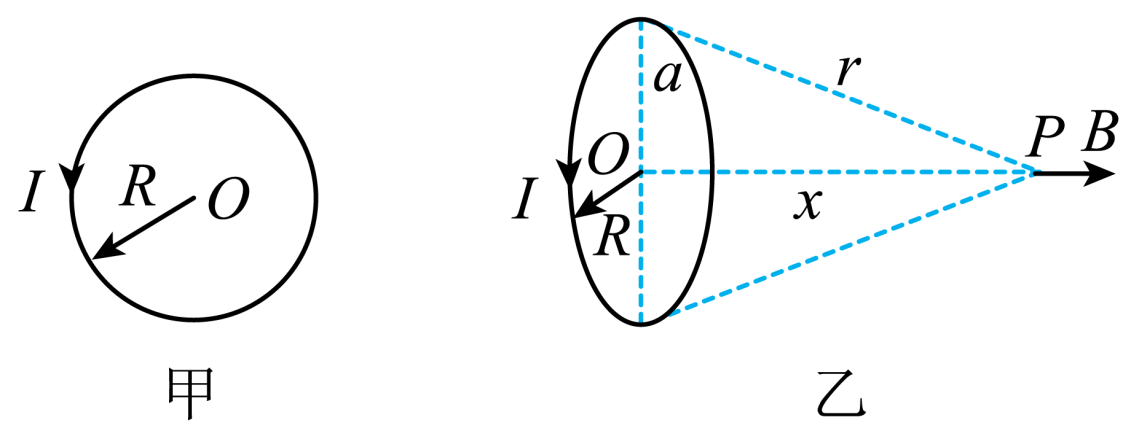
\includegraphics[width=0.6\textwidth]{fig/si_exercise_magfield_unit.png}
    \end{figure}
    \begin{tasks}(2)
        \task $B_P= \frac{\mu_{0}}{2}\cdot\frac{R^2 I}{\left( R^2 + x^2 \right)
        ^{3 / 2}}$
        \task $B_P= \frac{\mu_{0}}{2}\cdot\frac{R^2 I}{R^2 + x^2}$
        \task $B_P= \frac{\mu_{0}}{2}\cdot\frac{RI}{\left( R^2 + x^2 \right)^{3 
        / 2}}$
        \task $B_P= \frac{\mu_{0}}{2}\cdot\frac{R^3 I}{\left( R^2 + x^2 \right)
        ^{3 / 2}}$
    \end{tasks}
\end{exercises}

\section{物理中的标量和矢量}
